\lab{Applications}{RiverCrossing}{Transit time crossing a river}
\label{lab:rivercrossing}
\objective{Introductory lab discussing a classical calculus of variations problem: how is a river to be crossed in the shortest possible time? We will look at a numerical solution using the pseudospectral method. }

Suppose a boat is to be rowed across a river, from a point $A$ on one side of a river ($x=-1$), to a point $B$ on the other side ($x=1$). 
How is the boat to be steered to minimize the time required to cross the river? 

Let us consider a typical trajectory for the boat as it crosses the river. 
If we assume the boat moves at a constant speed 1 and let $T$ be the time required to cross the river, then the position $s(t)$ of the boat at time $t$ as it crosses the river is
\begin{align*}
	s(t) &= \langle x(t), y(t) \rangle, \quad t \in [0,T], \\
	s'(t) &= \langle x'(t), y'(t) \rangle, \\
	&= \langle \cos \sigma(x(t)),\sin \sigma(x(t)) \rangle + \langle 0, r(x(t)) \rangle.
\end{align*}
Here $\langle \cos \sigma, \sin \sigma \rangle$ represents the motion of the boat due to the rower, and $\langle 0, r \rangle$ is the motion of the boat due to the current.

We can relate the angle at which the boat is steered to the graph of its trajectory by noting that 
\begin{align*}
	y'(x) &= \frac{y'(t)}{x'(t)} ,\\
	&= \frac{\sin \sigma + r}{\cos \sigma},\\
	&= r\sec \sigma + \tan \sigma , \\
	&= r \sec \sigma + \sqrt{\sec^2 \sigma -1}.
\end{align*}
The time $T$ required to cross the river is given by
\begin{align*}
	T &= \int_{-1}^1 t'(x)\, dx, \\
	&= \int_{-1}^1 \frac{1}{x'(t)}\, dx \\ 
	&= \int_{-1}^1 \sec \sigma (x)\, dx. 
\end{align*}
We would like to find an expression for the total time $T$ required to cross the river from $A$ to $B$, in terms of the graph of the boat's trajectory. To derive the function $T[y]$, we note that 
\begin{align*}
	T[y] &= \int_{-1}^1 \sec \sigma\, dx,\\
	&= \int_{-1}^1 \frac{1}{1-r^2}(r \tan \sigma + \sec \sigma -r^2 \sec \sigma - r\tan \sigma)\, dx, \\
	&= \int_{-1}^1 \frac{1}{1-r^2}(r \tan \sigma + \sec \sigma -r(r \sec \sigma +\sqrt{\sec^2 \sigma - 1} ) )\, dx, \\
	&= \int_{-1}^1 \frac{1}{1-r^2}(r \tan \sigma + \sec \sigma -r y' )\, dx.	
\end{align*}
Since 
\begin{align*}
	r\tan \sigma  &= \sqrt{1 - r^2 + (r \sec \sigma + \tan \sigma)^2},\\
	&= \sqrt{1 - r^2 + (y')^2},
\end{align*}
we obtain at last
\begin{align}
	T[y] &= \int_{-1}^1 \left[ \alpha(x)\sqrt{1 + (\alpha y')^2(x)} - (\alpha^2 r y')(x) \right]\, dx,
\end{align}
where $\alpha = (1 - r^2)^{-1/2}$.

% Suppose that the graph of a function $y(x), \, x\in [-1,1]$ describes the path of the boat as it crosses a river. We assume that the speed at which the boat is rowed relative to the current remains constant. The time required for the boat to cross the river can be described by the functional 
% \begin{align*}
% T[y] &=  \int_{-1}^1 L(x,y,y')\, dx
% \end{align*}
% where 
% \begin{align*}
% 	L(x,y,y') &= \alpha(x) \sqrt{1 + \alpha^2(x)(y')^2} - \alpha^2(x)c(x)y', \\
% 	\alpha(x) &= (1-c^2(x))^{-1/2},
% \end{align*}
% and $c(x)$ is a known function that describes the current of the river at any point $x \in [-1,1]$. We will assume that the current is faster near the center of the river. 




We look for the path $y(x)$ that minimizes the time required for the boat to cross the river, so that the function $T$ is minimized. From the calculus of variations we know that a smooth path $y(x)$ minimizes $T$ only if the Euler-Lagrange equation is satisfied. Recall that the Euler-Lagrange equation is 
\[
% \frac{\partial }{\partial y}L - \frac{d}{dx}\frac{\partial }{\partial y'}L
L_{y} - \frac{d}{dx}L_{y'} = 0.
\]
% Since $L_y = 0,$ this problem is equivalent to solving the first order ordinary differential equation
% \begin{align*}
% 	L_{y'} = \alpha(x)(1 + \alpha^2 (y')^2)^{-1/2}\alpha^2 y' - \alpha^2 r =   k,
% \end{align*}
% where $k$ is some appropriately chosen constant. To help us choose integration constants, we will impose boundary conditions $y(-1) = 0$, $y(1) = y_1$. 



\begin{problem}
	Assume that $c(x)$ is given by $c(x) = -.5(x-1)(x+1)$.%, and $y(1) = y_1$.
	Write a Python function that accepts as arguments a function $y$ (or $y'$) and an $x$-value, and returns $L(x,y(x),y'(x))$. Use that function to define a second function that numerically computes $T[y]$ for a given path $y(x)$.
\end{problem}



\begin{figure}
\centering
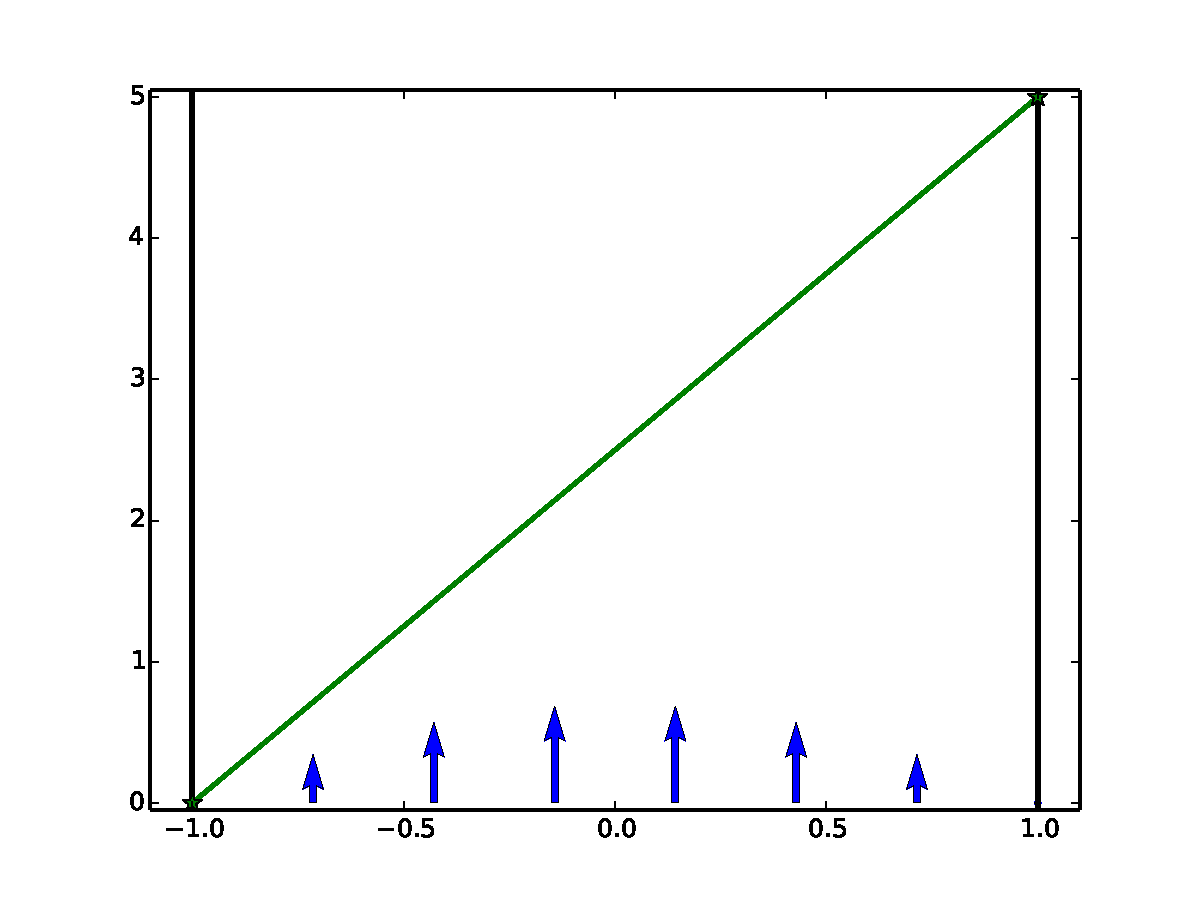
\includegraphics[width=\textwidth]{rivercurrent.pdf}
\caption{We will use the function $c(x) = -.5(x-1)(x+1)$ to describe the river's current.}
\label{fig:rivercrossing_current}
\end{figure}







